\documentclass[12pt,a4paper]{article}

% ─── Page Layout ───────────────────────────────────────────────────────────────
\usepackage[a4paper, margin=0.8in, headheight=14pt]{geometry}

% ─── Fonts (XeLaTeX) ───────────────────────────────────────────────────────────
\usepackage{fontspec}
\usepackage{unicode-math}
\setmainfont{TeX Gyre Pagella}
\setmonofont[Scale=0.88]{TeX Gyre Cursor}
\setmathfont{Latin Modern Math}

% ─── Packages ──────────────────────────────────────────────────────────────────
\usepackage{xcolor}
\usepackage{colortbl}
\usepackage{titlesec}
\usepackage{enumitem}
\usepackage{tabularx}
\usepackage{booktabs}
\usepackage{array}
\usepackage{amsmath}
\usepackage{tikz}
\usetikzlibrary{shapes.geometric, arrows.meta, positioning, calc, fit}
\usepackage{tcolorbox}
\tcbuselibrary{skins, breakable}
\usepackage{hyperref}
\usepackage{fancyhdr}
\usepackage{graphicx}
\usepackage{microtype}
\hyphenpenalty=10000
\exhyphenpenalty=10000
\sloppy
\usepackage{caption}
\usepackage{setspace}
\usepackage{multirow}
\usepackage{tocloft}

% ─── Q&A helper ────────────────────────────────────────────────────────────────
\newcommand{\Q}[1]{\textbf{#1}\par\noindent\ignorespaces}

% ─── Colour Palette ────────────────────────────────────────────────────────────
\definecolor{myred}{RGB}{196,30,58}
\definecolor{mydark}{RGB}{30,30,50}
\definecolor{mygreen}{RGB}{14,120,80}
\definecolor{myteal}{RGB}{0,130,140}
\definecolor{myamber}{RGB}{180,100,0}
\definecolor{mypurple}{RGB}{100,30,160}
\definecolor{mygray}{RGB}{246,247,249}
\definecolor{mgframe}{RGB}{180,185,200}
\definecolor{watermark}{RGB}{145,150,170}
\definecolor{hdrred}{RGB}{250,232,235}
\definecolor{hdrgreen}{RGB}{220,244,233}
\definecolor{hdrteal}{RGB}{220,242,244}
\definecolor{hdramber}{RGB}{253,242,215}
\definecolor{hdrpurple}{RGB}{238,228,255}
\definecolor{hdrgray}{RGB}{238,240,245}
\definecolor{rowalt}{RGB}{250,251,253}

% ─── Section Formatting ────────────────────────────────────────────────────────
\titleformat{\section}
  {\large\bfseries\color{myred}}{\thesection.}{0.5em}{}
  [\vspace{1pt}{\color{myred}\rule{\linewidth}{0.8pt}}]
\titleformat{\subsection}
  {\normalsize\bfseries\color{myteal}}{\thesubsection}{0.5em}{}
\titlespacing*{\section}{0pt}{18pt}{7pt}
\titlespacing*{\subsection}{0pt}{11pt}{4pt}
\setlength{\parindent}{0pt}
\setlength{\parskip}{4pt}

% ─── TOC Styling ───────────────────────────────────────────────────────────────
\renewcommand{\cfttoctitlefont}{\large\bfseries\color{myred}}
\renewcommand{\cftaftertoctitle}{\par\noindent{\color{myred}\rule{\linewidth}{0.8pt}}}
\setlength{\cftbeforetoctitleskip}{0pt}
\setlength{\cftaftertoctitleskip}{6pt}
\renewcommand{\cftsecfont}{\normalsize\bfseries\color{mydark}}
\renewcommand{\cftsecpagefont}{\normalsize\bfseries\color{mydark}}
\renewcommand{\cftsecleader}{\cftdotfill{\cftdotsep}}
\setlength{\cftbeforesecskip}{7pt}
\renewcommand{\cftsubsecfont}{\small\color{mydark}}
\renewcommand{\cftsubsecpagefont}{\small\color{mydark}}
\setlength{\cftbeforesubsecskip}{3pt}
\setlength{\cftsubsecindent}{1.4em}

% ─── Table helpers ─────────────────────────────────────────────────────────────
\renewcommand{\arraystretch}{1.45}
\setlength{\tabcolsep}{6pt}
\arrayrulecolor{mydark}
\newcolumntype{B}[1]{>{\small\bfseries\raggedright\arraybackslash}m{#1}}
\newcolumntype{Y}{>{\small\raggedright\arraybackslash}X}
\renewcommand{\tabularxcolumn}[1]{m{#1}}

% ─── Header / Footer ───────────────────────────────────────────────────────────
\pagestyle{fancy}
\fancyhf{}
\fancyhead[L]{\small\color{myred}\textbf{EC602}\;\color{mydark}--- Computer Network}
\fancyhead[R]{\small\color{myteal}\textbf{Module 4 Notes}}
\fancyfoot[C]{\small\color{mydark}\thepage}
\fancyfoot[R]{\small\color{watermark}\textit{\copyright\ Biraj}}
\renewcommand{\headrulewidth}{0.5pt}
\renewcommand{\footrulewidth}{0.3pt}

% ─── Hyperref ──────────────────────────────────────────────────────────────────
\hypersetup{
  colorlinks=true, linkcolor=myteal, urlcolor=myteal,
  pdfauthor={Biraj Sarkar},
  pdftitle={EC602 --- Module 4 Notes}
}

% ─── tcolorbox styles ──────────────────────────────────────────────────────────
\tcbset{
  tikzbox/.style={colback=mygray, colframe=mgframe, boxrule=0.6pt, arc=4pt,
    left=8pt, right=8pt, top=6pt, bottom=6pt,
    colbacktitle=mgframe, coltitle=mydark, fonttitle=\small\bfseries},
  defbox/.style={colback=hdrgreen, colframe=mygreen, boxrule=0.8pt, arc=4pt,
    left=9pt, right=9pt, top=6pt, bottom=6pt,
    colbacktitle=mygreen, coltitle=white, fonttitle=\small\bfseries},
  formulabox/.style={colback=hdrteal, colframe=myteal, boxrule=0.8pt, arc=4pt,
    left=9pt, right=9pt, top=7pt, bottom=7pt,
    colbacktitle=myteal, coltitle=white, fonttitle=\small\bfseries},
  examplebox/.style={colback=hdramber, colframe=myamber, boxrule=0.8pt, arc=4pt,
    left=9pt, right=9pt, top=6pt, bottom=6pt,
    colbacktitle=myamber, coltitle=white, fonttitle=\small\bfseries},
  masonbox/.style={colback=hdrpurple, colframe=mypurple, boxrule=0.8pt, arc=4pt,
    left=9pt, right=9pt, top=6pt, bottom=6pt,
    colbacktitle=mypurple, coltitle=white, fonttitle=\small\bfseries},
  exambox/.style={colback=hdrpurple, colframe=mypurple, boxrule=1pt, arc=5pt,
    left=10pt, right=10pt, top=8pt, bottom=8pt,
    colbacktitle=mypurple, coltitle=white, fonttitle=\bfseries,
    breakable}
}
% Make all boxes breakable across pages
\tcbset{breakable}

\tikzset{
  block/.style={rectangle, draw=myteal, fill=hdrteal, text width=2.2cm, align=center,
    minimum height=0.85cm, font=\small, rounded corners=3pt, line width=0.7pt},
  arrow/.style={-Stealth, thick, color=mydark},
  line/.style={thick, color=mydark}
}

% ═══════════════════════════════════════════════════════════════════════════════
\begin{document}
% ═══════════════════════════════════════════════════════════════════════════════

\begin{center}
  {\LARGE\bfseries\color{myred} EC602 --- Computer Network}\\[5pt]
  {\normalsize\color{mydark} Semester VI \quad$\bullet$\quad 3L:0T:0P \quad$\bullet$\quad 3 Credits}\\[3pt]
  {\normalsize\color{myteal}\textbf{Module 4 Exam Notes}}\\[3pt]
  {\small\color{mydark} CGEC \;$|$\; B.Tech ECE (2023--27) \;$|$\; \textit{Biraj Sarkar}}
\end{center}
\vspace{2pt}
\noindent{\color{myred}\rule{\linewidth}{1.5pt}}
\vspace{2pt}
\hypersetup{linkcolor=mydark}
\tableofcontents
\hypersetup{linkcolor=myteal}
\newpage

%═══════════════════════════════════════════════════════════════════════════════
\section{Application Layer Protocols}
%═══════════════════════════════════════════════════════════════════════════════

\begin{tcolorbox}[defbox]
\textbf{Application Layer (Layer 7):} Provides network services directly to user applications. Protocols define the format and rules for communication between applications on different hosts.
\end{tcolorbox}

\begin{tabularx}{\linewidth}{|B{2.4cm}|>{\centering\arraybackslash}p{1.8cm}|>{\centering\arraybackslash}p{2.0cm}|X|}
\hline
\multicolumn{1}{|>{\centering\arraybackslash}p{2.4cm}|}{\textbf{\color{myteal}Protocol}} &
\textbf{\color{myteal}Port} &
\textbf{\color{myteal}Transport} &
\multicolumn{1}{>{\centering\arraybackslash}X|}{\textbf{\color{myteal}Function}} \\
\hline
DNS  & 53  & UDP/TCP & Resolves domain names to IP addresses. \\
\hline
SMTP & 25  & TCP     & Sends email from client to server (or server to server). \\
\hline
SNMP & 161 & UDP     & Manages and monitors network devices. \\
\hline
FTP  & 20/21 & TCP   & File transfer; port 21 = control, port 20 = data. \\
\hline
HTTP & 80  & TCP     & Transfers web pages (HyperText Transfer Protocol). \\
\hline
HTTPS& 443 & TCP     & Secure HTTP using TLS/SSL encryption. \\
\hline
\end{tabularx}

\subsection{DNS (Domain Name System)}

\begin{tcolorbox}[formulabox, title={\textbf{DNS}}]
\textbf{Function:} Translates human-readable domain names (e.g.\ \texttt{www.google.com}) to IP addresses.\\
\textbf{Hierarchy:} Root DNS $\to$ TLD servers (.com, .org, .in) $\to$ Authoritative DNS servers.\\
\textbf{Resolution types:}
\begin{itemize}[leftmargin=*, itemsep=2pt, topsep=0pt]
  \item \textbf{Recursive:} DNS resolver queries on behalf of client until answer found.
  \item \textbf{Iterative:} DNS server returns best referral; client queries next server itself.
\end{itemize}
\textbf{Caching:} DNS responses cached with TTL to reduce lookup time.
\end{tcolorbox}

\begin{tcolorbox}[tikzbox, title={DNS Resolution Hierarchy}]
\centering
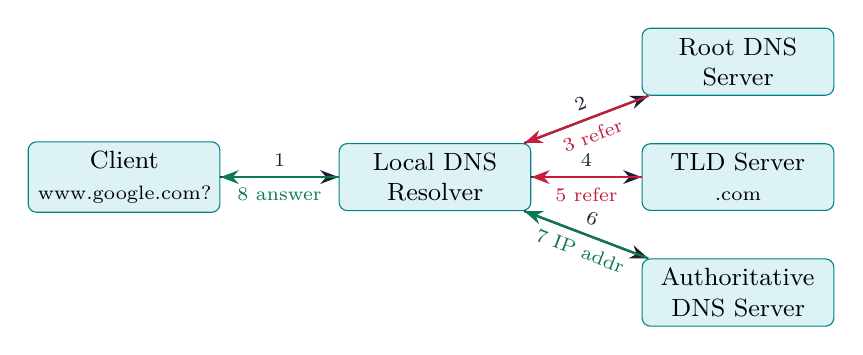
\begin{tikzpicture}[
  srv/.style={rectangle, draw=myteal, fill=hdrteal, text width=2.2cm, align=center, minimum height=0.65cm, font=\small, rounded corners=3pt},
  node distance=0.5cm
]
\node[srv] (client) {Client\\{\scriptsize www.google.com?}};
\node[srv, right=1.5cm of client] (resolver) {Local DNS\\Resolver};
\node[srv, above right=0.6cm and 1.4cm of resolver] (root) {Root DNS\\Server};
\node[srv, right=1.4cm of resolver] (tld) {TLD Server\\{\scriptsize .com}};
\node[srv, below right=0.6cm and 1.4cm of resolver] (auth) {Authoritative\\DNS Server};

\draw[arrow] (client) -- node[above]{\scriptsize 1} (resolver);
\draw[arrow] (resolver) -- node[above,sloped]{\scriptsize 2} (root);
\draw[arrow,color=myred] (root) -- node[below,sloped]{\scriptsize 3 refer} (resolver);
\draw[arrow] (resolver) -- node[above]{\scriptsize 4} (tld);
\draw[arrow,color=myred] (tld) -- node[below]{\scriptsize 5 refer} (resolver);
\draw[arrow] (resolver) -- node[above,sloped]{\scriptsize 6} (auth);
\draw[arrow,color=mygreen] (auth) -- node[below,sloped]{\scriptsize 7 IP addr} (resolver);
\draw[arrow,color=mygreen] (resolver) -- node[below]{\scriptsize 8 answer} (client);
\end{tikzpicture}
\end{tcolorbox}

\subsection{HTTP and WWW}

\begin{tcolorbox}[defbox]
\textbf{HTTP (HyperText Transfer Protocol):} Application layer protocol for transferring web content. Stateless, request-response model. Client sends HTTP request; server responds with status code and content.
\end{tcolorbox}

\textbf{HTTP Methods:} GET (retrieve), POST (submit data), PUT (update), DELETE (remove), HEAD (headers only).\\
\textbf{Common Status Codes:} 200 OK, 301 Moved Permanently, 404 Not Found, 500 Internal Server Error.\\
\textbf{WWW:} World Wide Web --- a system of interlinked hypertext documents accessed via HTTP. Uses URLs, HTML, and browsers.

%═══════════════════════════════════════════════════════════════════════════════
\section{Network Security}
%═══════════════════════════════════════════════════════════════════════════════

\subsection{Cryptography}

\begin{tcolorbox}[defbox]
\textbf{Cryptography:} The science of securing information by transforming it into an unreadable format (ciphertext) using an algorithm and a key. Only authorised parties with the correct key can decrypt it.
\end{tcolorbox}

\subsubsection*{Symmetric Key (Private Key) Cryptography}
\begin{tcolorbox}[formulabox, title={\textbf{Symmetric Key Cryptography}}]
\textbf{Concept:} Same key used for both encryption and decryption. Both sender and receiver must share the secret key securely.\\[4pt]
\textbf{Algorithms:} DES (56-bit key), 3DES, AES (128/192/256-bit), RC4, Blowfish.\\[4pt]
\textbf{Advantages:} Fast, low computational overhead, suitable for bulk data encryption.\\
\textbf{Disadvantages:} Key distribution problem --- how to securely share the key? Does not scale well ($n$ users need $n(n-1)/2$ keys).
\end{tcolorbox}

\subsubsection*{Asymmetric Key (Public Key) Cryptography}
\begin{tcolorbox}[formulabox, title={\textbf{Asymmetric Key Cryptography}}]
\textbf{Concept:} Uses a \textbf{key pair} --- a \textbf{public key} (shared openly) and a \textbf{private key} (kept secret). Data encrypted with public key can only be decrypted with the corresponding private key.\\[4pt]
\textbf{Algorithms:} RSA, Diffie-Hellman, ECC (Elliptic Curve Cryptography).\\[4pt]
\textbf{Encryption:} Sender encrypts with receiver's \textbf{public key}; receiver decrypts with \textbf{private key}.\\
\textbf{Advantages:} Solves key distribution problem; enables digital signatures.\\
\textbf{Disadvantages:} Computationally expensive; much slower than symmetric encryption.
\end{tcolorbox}

\begin{tabularx}{\linewidth}{|B{3.0cm}|X|X|}
\hline
\multicolumn{1}{|>{\centering\arraybackslash}p{3.0cm}|}{\textbf{Feature}} &
\multicolumn{1}{>{\centering\arraybackslash}X|}{\textbf{\color{myteal}Symmetric}} &
\multicolumn{1}{>{\centering\arraybackslash}X|}{\textbf{\color{myamber}Asymmetric}} \\
\hline
Keys used       & Same key (shared secret)      & Public + Private key pair \\
\hline
Speed           & Fast                          & Slow \\
\hline
Key distribution& Difficult (must share secretly)& Easy (public key is open) \\
\hline
Scalability     & Poor ($n^2/2$ keys)           & Good ($2n$ keys for $n$ users) \\
\hline
Examples        & AES, DES, RC4                 & RSA, Diffie-Hellman, ECC \\
\hline
Use case        & Bulk data encryption          & Key exchange, digital signatures \\
\hline
\end{tabularx}

\subsection{Digital Signature}

\begin{tcolorbox}[defbox]
\textbf{Digital Signature:} A cryptographic mechanism that provides \textbf{authentication}, \textbf{integrity}, and \textbf{non-repudiation}. Created by encrypting a message digest (hash) with the sender's \textbf{private key}.
\end{tcolorbox}

\textbf{Process:}
\begin{enumerate}[label=\textbf{\arabic*.}, leftmargin=*, itemsep=3pt]
  \item Sender computes hash of message using a hash function (e.g.\ SHA-256).
  \item Sender encrypts the hash with their \textbf{private key} --- this is the digital signature.
  \item Receiver decrypts the signature using sender's \textbf{public key} to get the hash.
  \item Receiver independently computes hash of received message.
  \item If both hashes match: message is authentic and unaltered.
\end{enumerate}

\begin{tcolorbox}[tikzbox, title={Digital Signature --- Sign \& Verify}]
\centering
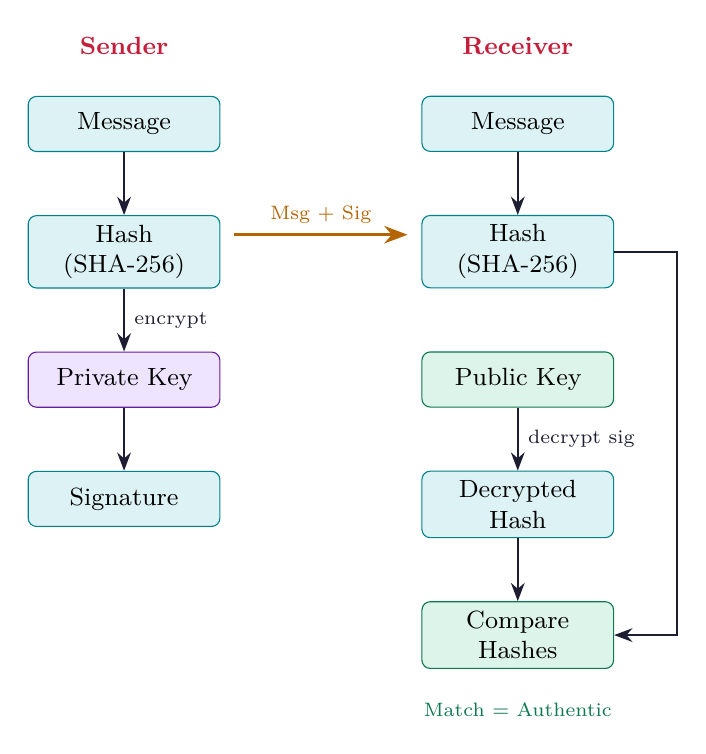
\begin{tikzpicture}[
  proc/.style={rectangle, draw=myteal, fill=hdrteal, text width=2.2cm, align=center, minimum height=0.7cm, font=\small, rounded corners=3pt},
  pkey/.style={rectangle, draw=mypurple, fill=hdrpurple, text width=2.2cm, align=center, minimum height=0.7cm, font=\small, rounded corners=3pt},
  gkey/.style={rectangle, draw=mygreen, fill=hdrgreen, text width=2.2cm, align=center, minimum height=0.7cm, font=\small, rounded corners=3pt},
  arr/.style={-Stealth, thick, color=mydark}
]
%--- SENDER column ---
\node[font=\small\bfseries\color{myred}] (slbl) at (1.1, 0.0) {Sender};
\node[proc,  below=0.4cm of slbl]  (msg1)  {Message};
\node[proc,  below=0.8cm of msg1]  (hash1) {Hash (SHA-256)};
\node[pkey,  below=0.8cm of hash1] (priv)  {Private Key};
\node[proc,  below=0.8cm of priv]  (sig)   {Signature};
\draw[arr] (msg1)  -- (hash1);
\draw[arr] (hash1) -- node[right, font=\scriptsize] {encrypt} (priv);
\draw[arr] (priv)  -- (sig);

%--- transfer arrow (horizontal, between columns) ---
\draw[-Stealth, very thick, color=myamber]
  (2.5, -2.4) -- node[above, font=\scriptsize\color{myamber}] {Msg + Sig} (4.7, -2.4);

%--- RECEIVER column ---
\node[font=\small\bfseries\color{myred}] (rlbl) at (6.1, 0.0) {Receiver};
\node[proc,  below=0.4cm of rlbl]  (msg2)  {Message};
\node[proc,  below=0.8cm of msg2]  (hash2) {Hash (SHA-256)};
\node[gkey,  below=0.8cm of hash2] (pub)   {Public Key};
\node[proc,  below=0.8cm of pub]   (dhash) {Decrypted Hash};
\node[gkey,  below=0.8cm of dhash] (cmp)   {Compare Hashes};
\draw[arr] (msg2)  -- (hash2);
\draw[arr] (pub)   -- node[right, font=\scriptsize] {decrypt sig} (dhash);
\draw[arr] (dhash) -- (cmp);
% hash2 feeds into compare via right side detour
\draw[arr] (hash2.east) -- ++(0.8,0) |- (cmp.east);

\node[font=\scriptsize\color{mygreen}, below=0.3cm of cmp] {Match = Authentic};
\end{tikzpicture}
\end{tcolorbox}

\subsection{Firewalls}

\begin{tcolorbox}[defbox]
\textbf{Firewall:} A network security device (hardware or software) that monitors and controls incoming/outgoing network traffic based on predefined security rules. Acts as a barrier between trusted internal network and untrusted external network.
\end{tcolorbox}

\textbf{Types of Firewalls:}\par\noindent
\begin{tabularx}{\linewidth}{|B{3.2cm}|X|}
\hline
\multicolumn{1}{|>{\centering\arraybackslash}p{3.2cm}|}{\textbf{\color{mygreen}Type}} &
\multicolumn{1}{>{\centering\arraybackslash}X|}{\textbf{\color{mygreen}Description}} \\
\hline
Packet Filter      & Inspects packets at network layer; filters based on IP, port, protocol. Stateless. \\
\hline
Stateful Inspection& Tracks connection state; allows only packets belonging to established connections. \\
\hline
Application Gateway& Proxy-based; inspects application layer data (HTTP, FTP). Most secure but slowest. \\
\hline
Circuit-level Gateway & Monitors TCP handshake; does not inspect packet content. \\
\hline
\end{tabularx}

\begin{tcolorbox}[tikzbox, title={Firewall Placement in a Network}]
\centering
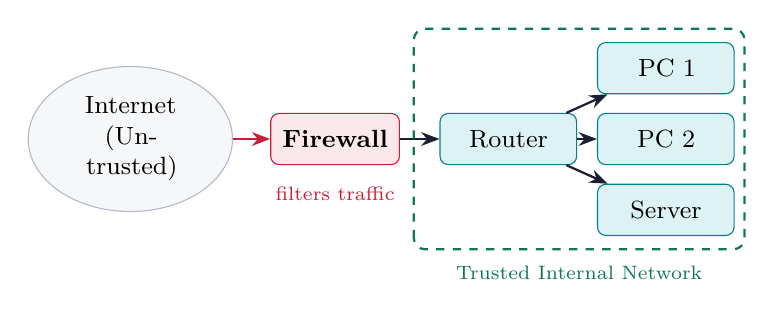
\begin{tikzpicture}[
  dev/.style={rectangle, draw=myteal, fill=hdrteal, text width=1.5cm, align=center, minimum height=0.65cm, font=\small, rounded corners=3pt},
  fw/.style={rectangle, draw=myred, fill=hdrred, text width=1.4cm, align=center, minimum height=0.65cm, font=\small\bfseries, rounded corners=3pt},
  cloud/.style={ellipse, draw=mgframe, fill=mygray, text width=1.6cm, align=center, font=\small}
]
\node[cloud] (inet)   at (0, 0)    {Internet\\(Untrusted)};
\node[fw]    (fw)     at (2.6, 0)  {Firewall};
\node[dev]   (router) at (4.8, 0)  {Router};
\node[dev]   (pc1)    at (6.8, 0.9){PC 1};
\node[dev]   (pc2)    at (6.8, 0)  {PC 2};
\node[dev]   (server) at (6.8,-0.9){Server};

\draw[arrow, color=myred] (inet)   -- (fw);
\draw[arrow]              (fw)     -- (router);
\draw[arrow]              (router) -- (pc1);
\draw[arrow]              (router) -- (pc2);
\draw[arrow]              (router) -- (server);

% dashed trusted zone box
\draw[dashed, color=mygreen, thick, rounded corners=4pt]
  (3.6, -1.4) rectangle (7.8, 1.4);
\node[font=\scriptsize\color{mygreen}] at (5.7, -1.7) {Trusted Internal Network};

% firewall label below fw node
\node[font=\scriptsize\color{myred}, below=0.15cm of fw] {filters traffic};
\end{tikzpicture}
\end{tcolorbox}

%═══════════════════════════════════════════════════════════════════════════════
\section{Modern Topics}
%═══════════════════════════════════════════════════════════════════════════════

\subsection{ISDN (Integrated Services Digital Network)}

\begin{tcolorbox}[defbox]
\textbf{ISDN:} A set of communication standards for simultaneous digital transmission of voice, video, data, and other services over traditional telephone copper wire. Replaced by DSL and broadband.
\end{tcolorbox}

\textbf{ISDN Channels:}
\begin{itemize}[leftmargin=*, itemsep=3pt]
  \item \textbf{B channel (Bearer):} 64 Kbps; carries user data (voice, video, data).
  \item \textbf{D channel (Delta):} 16 or 64 Kbps; carries signalling and control information.
\end{itemize}

\textbf{ISDN Interfaces:}\par\noindent
\begin{tabularx}{\linewidth}{|B{2.8cm}|X|}
\hline
\multicolumn{1}{|>{\centering\arraybackslash}p{2.8cm}|}{\textbf{\color{myteal}Interface}} &
\multicolumn{1}{>{\centering\arraybackslash}X|}{\textbf{\color{myteal}Description}} \\
\hline
BRI (Basic Rate)   & $2B + D$ = $2 \times 64$ Kbps + 16 Kbps D = 144 Kbps. For home/small office. \\
\hline
PRI (Primary Rate) & $23B + D$ (North America) or $30B + D$ (Europe) = 1.544 / 2.048 Mbps. For enterprises. \\
\hline
\end{tabularx}

\subsection{ATM (Asynchronous Transfer Mode)}

\begin{tcolorbox}[defbox]
\textbf{ATM:} A cell-switching and multiplexing technology that uses fixed-size \textbf{53-byte cells} (5-byte header + 48-byte payload) for transmitting voice, video, and data over high-speed networks.
\end{tcolorbox}

\textbf{Key Features:}
\begin{itemize}[leftmargin=*, itemsep=3pt]
  \item Fixed 53-byte cells enable predictable, low-latency switching.
  \item Connection-oriented: virtual circuits (VC) established before data transfer.
  \item Supports QoS guarantees for different traffic types (CBR, VBR, ABR, UBR).
  \item \textbf{VPI/VCI:} Virtual Path Identifier / Virtual Channel Identifier used for routing cells.
\end{itemize}

\subsection{DSL (Digital Subscriber Line)}

\begin{tcolorbox}[defbox]
\textbf{DSL:} A family of technologies that transmit digital data over existing telephone copper wire pairs at high speeds. Uses frequencies above the voice band (above 4 kHz).
\end{tcolorbox}

\begin{tabularx}{\linewidth}{|B{2.8cm}|X|X|}
\hline
\multicolumn{1}{|>{\centering\arraybackslash}p{2.8cm}|}{\textbf{Type}} &
\multicolumn{1}{>{\centering\arraybackslash}X|}{\textbf{Speed}} &
\multicolumn{1}{>{\centering\arraybackslash}X|}{\textbf{Description}} \\
\hline
ADSL (Asymmetric)  & Down: 8 Mbps, Up: 1 Mbps & Different download/upload speeds. Most common for home use. \\
\hline
SDSL (Symmetric)   & 2 Mbps both ways          & Equal upload/download. Used by businesses. \\
\hline
VDSL (Very High)   & Down: 52 Mbps, Up: 16 Mbps & Very high speed over short distances. \\
\hline
\end{tabularx}

\textbf{DSL Modem:} Connects user's equipment to the telephone line. Separates voice (0--4 kHz) and data (above 4 kHz) using a \textbf{splitter}.

\subsection{Cable Modem}

\begin{tcolorbox}[defbox]
\textbf{Cable Modem:} A device that provides Internet access over the cable TV (CATV) infrastructure using coaxial cable. Uses \textbf{DOCSIS} (Data Over Cable Service Interface Specification) standard.
\end{tcolorbox}

\textbf{Key Points:}
\begin{itemize}[leftmargin=*, itemsep=3pt]
  \item Shared medium: all users in a neighbourhood share the same cable segment (bandwidth shared).
  \item Downstream (TV to user): 6 MHz channel, up to 30--40 Mbps.
  \item Upstream (user to TV headend): narrower band, typically 5--42 MHz.
  \item \textbf{HFC (Hybrid Fibre-Coaxial):} Fibre from headend to neighbourhood node; coaxial to homes.
\end{itemize}

\subsection{Wireless LAN --- IEEE 802.11}

\begin{tcolorbox}[defbox]
\textbf{IEEE 802.11 (Wi-Fi):} A set of standards for wireless local area networking. Uses radio frequencies (2.4 GHz and 5 GHz bands). MAC protocol: CSMA/CA.
\end{tcolorbox}

\textbf{IEEE 802.11 Standards:}\par\noindent
\begin{tabularx}{\linewidth}{|>{\centering\arraybackslash}p{2.0cm}|>{\centering\arraybackslash}p{2.0cm}|>{\centering\arraybackslash}p{2.4cm}|X|}
\hline
\textbf{\color{myteal}Standard} & \textbf{\color{myteal}Year} & \textbf{\color{myteal}Frequency} & \multicolumn{1}{>{\centering\arraybackslash}X|}{\textbf{\color{myteal}Max Speed}} \\
\hline
802.11b & 1999 & 2.4 GHz & 11 Mbps \\
\hline
802.11a & 1999 & 5 GHz   & 54 Mbps \\
\hline
802.11g & 2003 & 2.4 GHz & 54 Mbps \\
\hline
802.11n & 2009 & 2.4/5 GHz & 600 Mbps (MIMO) \\
\hline
802.11ac& 2013 & 5 GHz   & 1+ Gbps \\
\hline
\end{tabularx}

\textbf{Architecture:}
\begin{itemize}[leftmargin=*, itemsep=3pt]
  \item \textbf{Infrastructure mode:} Devices connect through an \textbf{Access Point (AP)}. AP connects to wired network. Most common.
  \item \textbf{Ad-hoc mode:} Devices communicate directly without an AP (peer-to-peer).
  \item \textbf{BSS (Basic Service Set):} Single AP + associated stations.
  \item \textbf{ESS (Extended Service Set):} Multiple BSSs connected via a distribution system.
\end{itemize}

\textbf{Security:} WEP (weak, deprecated) $\to$ WPA $\to$ WPA2 (AES-based, current standard) $\to$ WPA3.

\subsection{Bluetooth}

\begin{tcolorbox}[defbox]
\textbf{Bluetooth (IEEE 802.15.1):} A short-range wireless technology for personal area networks (PAN). Operates at 2.4 GHz ISM band. Range: $\sim$10 m (Class 2). Uses \textbf{FHSS} (Frequency Hopping Spread Spectrum) --- hops 1600 times/second across 79 channels.
\end{tcolorbox}

\textbf{Bluetooth Network (Piconet):}
\begin{itemize}[leftmargin=*, itemsep=3pt]
  \item \textbf{Piconet:} One \textbf{master} + up to 7 active \textbf{slaves}. Master controls timing and frequency hopping.
  \item \textbf{Scatternet:} Multiple overlapping piconets; a device can be slave in multiple piconets or master in one and slave in another.
\end{itemize}

\begin{tcolorbox}[tikzbox, title={Bluetooth Piconet Structure}]
\centering
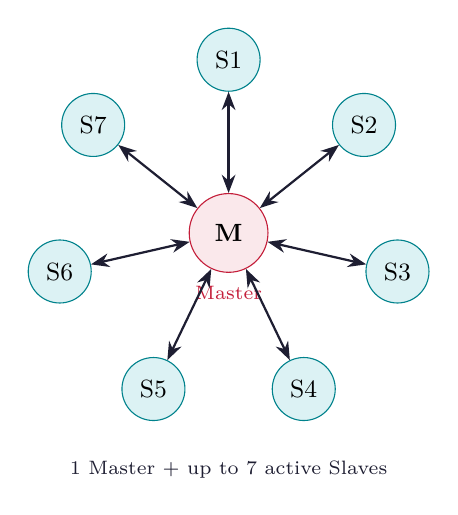
\begin{tikzpicture}[
  master/.style={circle, draw=myred, fill=hdrred, minimum size=1.0cm, font=\small\bfseries, align=center},
  slave/.style={circle, draw=myteal, fill=hdrteal, minimum size=0.8cm, font=\small, align=center}
]
\node[master] (M) {M};
\node[font=\scriptsize\color{myred}, below=0.05cm of M] {Master};
\foreach \i/\lbl in {1/S1, 2/S2, 3/S3, 4/S4, 5/S5, 6/S6, 7/S7} {
  \pgfmathsetmacro\ang{90 - (\i-1)*360/7}
  \node[slave] (S\i) at (\ang:2.2cm) {\lbl};
  \draw[thick, color=mydark, <->, >=Stealth] (M) -- (S\i);
}
\node[font=\scriptsize\color{mydark}] at (0,-3.0) {1 Master + up to 7 active Slaves};
\end{tikzpicture}
\end{tcolorbox}

\textbf{Bluetooth Versions:}\par\noindent
\begin{tabularx}{\linewidth}{|>{\centering\arraybackslash}p{2.2cm}|X|}
\hline
\textbf{\color{myteal}Version} & \multicolumn{1}{>{\centering\arraybackslash}X|}{\textbf{\color{myteal}Key Feature}} \\
\hline
1.2  & Basic rate 1 Mbps; AFH (Adaptive Frequency Hopping) \\
\hline
2.0 + EDR & Enhanced Data Rate; up to 3 Mbps \\
\hline
4.0 (BLE) & Bluetooth Low Energy; very low power; IoT devices \\
\hline
5.0  & 2$\times$ speed, 4$\times$ range, 8$\times$ broadcast capacity vs.\ 4.2 \\
\hline
\end{tabularx}

%═══════════════════════════════════════════════════════════════════════════════
% QUICK REVISION PAGE
%═══════════════════════════════════════════════════════════════════════════════
\newpage
\begin{center}
  {\large\bfseries\color{myred} Quick Revision --- Module 4}\\[3pt]
  {\small\color{mydark} Application Layer, Security \& Modern Topics $|$ EC602}
\end{center}
\noindent{\color{myred}\rule{\linewidth}{1.2pt}}
\vspace{4pt}

\begin{tcolorbox}[formulabox, title={\textbf{Key Facts at a Glance}}]
\begin{tabularx}{\linewidth}{B{5.0cm} X}
DNS port            & 53 (UDP/TCP) \\[2pt]
SMTP port           & 25 (TCP) \\[2pt]
FTP ports           & 21 (control), 20 (data) \\[2pt]
HTTP / HTTPS ports  & 80 / 443 \\[2pt]
SNMP port           & 161 (UDP) \\[2pt]
Symmetric key       & Same key for encrypt/decrypt (AES, DES) \\[2pt]
Asymmetric key      & Public key encrypts; private key decrypts (RSA) \\[2pt]
Digital signature   & Hash encrypted with sender's private key \\[2pt]
ISDN BRI            & $2B + D$ = 144 Kbps \\[2pt]
ISDN PRI (Europe)   & $30B + D$ = 2.048 Mbps \\[2pt]
ATM cell size       & 53 bytes (5 header + 48 payload) \\[2pt]
ADSL speed          & Down 8 Mbps / Up 1 Mbps \\[2pt]
802.11b speed       & 11 Mbps @ 2.4 GHz \\[2pt]
802.11g/a speed     & 54 Mbps \\[2pt]
Bluetooth range     & $\sim$10 m; 2.4 GHz; FHSS; 1600 hops/sec \\[2pt]
Piconet             & 1 master + up to 7 active slaves \\[2pt]
\end{tabularx}
\end{tcolorbox}

\vspace{6pt}

\begin{tcolorbox}[defbox, title={\textbf{One-Line Definitions}}]
\begin{itemize}[leftmargin=*, itemsep=3pt, topsep=0pt]
  \item \textbf{DNS:} Translates domain names to IP addresses using a hierarchical distributed database.
  \item \textbf{HTTP:} Stateless request-response protocol for transferring web content.
  \item \textbf{SMTP:} Protocol for sending email between mail servers.
  \item \textbf{FTP:} Protocol for transferring files; uses separate control (21) and data (20) connections.
  \item \textbf{Symmetric Cryptography:} Same secret key used for both encryption and decryption.
  \item \textbf{Asymmetric Cryptography:} Public key encrypts; private key decrypts (or vice versa for signatures).
  \item \textbf{Digital Signature:} Hash of message encrypted with sender's private key; proves authenticity.
  \item \textbf{Firewall:} Security device that filters network traffic based on rules.
  \item \textbf{ISDN:} Digital telephone network supporting voice, video, and data simultaneously.
  \item \textbf{ATM:} Cell-switching technology using fixed 53-byte cells; supports QoS.
  \item \textbf{DSL:} High-speed Internet over telephone copper wire using frequencies above voice band.
  \item \textbf{IEEE 802.11:} Wi-Fi standard; uses CSMA/CA; operates at 2.4/5 GHz.
  \item \textbf{Bluetooth:} Short-range PAN technology; 2.4 GHz; FHSS; piconet architecture.
\end{itemize}
\end{tcolorbox}

\vspace{6pt}

\begin{tcolorbox}[exambox, title={\textbf{Frequently Asked / Viva Questions}}]
\begin{enumerate}[leftmargin=*, topsep=0pt, label=\textbf{Q\arabic*.}, itemsep=8pt]
  \item \Q{What is DNS and how does it work?} DNS translates domain names to IP addresses. Client queries local DNS resolver; if not cached, resolver queries root $\to$ TLD $\to$ authoritative DNS servers recursively or iteratively.
  \item \Q{What is the difference between symmetric and asymmetric cryptography?} Symmetric: same key for encrypt/decrypt, fast, key distribution problem. Asymmetric: public/private key pair, slower, solves key distribution.
  \item \Q{How does a digital signature work?} Sender hashes the message and encrypts the hash with their private key. Receiver decrypts with sender's public key and compares hashes to verify authenticity and integrity.
  \item \Q{What is a firewall?} A security device that monitors and filters network traffic based on predefined rules, acting as a barrier between trusted and untrusted networks.
  \item \Q{What is the difference between packet filter and stateful firewall?} Packet filter: stateless, inspects each packet independently. Stateful: tracks connection state, allows only packets belonging to established connections.
  \item \Q{What is ATM and what is its cell size?} Asynchronous Transfer Mode; cell-switching technology using fixed 53-byte cells (5-byte header + 48-byte payload).
  \item \Q{What is ADSL?} Asymmetric DSL; provides higher download speed (up to 8 Mbps) than upload speed (up to 1 Mbps) over telephone copper wire.
  \item \Q{What MAC protocol does IEEE 802.11 use?} CSMA/CA (Carrier Sense Multiple Access with Collision Avoidance).
  \item \Q{What is a piconet in Bluetooth?} A small network of one master and up to 7 active slave devices communicating on the same frequency hopping sequence.
  \item \Q{What is FHSS in Bluetooth?} Frequency Hopping Spread Spectrum; Bluetooth hops across 79 channels 1600 times per second to reduce interference and improve security.
  \item \Q{What is the difference between infrastructure and ad-hoc Wi-Fi mode?} Infrastructure: devices connect through an Access Point. Ad-hoc: devices communicate directly without an AP.
  \item \Q{What is ISDN BRI?} Basic Rate Interface: $2B + D$ channels = $2 \times 64$ Kbps + 16 Kbps = 144 Kbps total. Used for home/small office ISDN connections.
\end{enumerate}
\end{tcolorbox}

\vspace{6pt}

\begin{tcolorbox}[tikzbox, title={\textbf{Application Layer Protocols Summary}}]
\begin{tabularx}{\linewidth}{|B{2.4cm}|>{\centering\arraybackslash}p{1.6cm}|>{\centering\arraybackslash}p{1.8cm}|X|}
\hline
\textbf{Protocol} & \textbf{Port} & \textbf{Transport} & \textbf{Purpose} \\
\hline
DNS  & 53  & UDP/TCP & Name resolution \\
\hline
SMTP & 25  & TCP & Send email \\
\hline
FTP  & 20/21 & TCP & File transfer \\
\hline
HTTP & 80  & TCP & Web pages \\
\hline
HTTPS& 443 & TCP & Secure web \\
\hline
SNMP & 161 & UDP & Network management \\
\hline
\end{tabularx}
\end{tcolorbox}

\end{document}
